\documentclass[14pt]{extbook}
\usepackage{multicol, enumerate, enumitem, hyperref, color, soul, setspace, parskip, fancyhdr} %General Packages
\usepackage{amssymb, amsthm, amsmath, latexsym, units, mathtools} %Math Packages
\everymath{\displaystyle} %All math in Display Style
% Packages with additional options
\usepackage[headsep=0.5cm,headheight=12pt, left=1 in,right= 1 in,top= 1 in,bottom= 1 in]{geometry}
\usepackage[usenames,dvipsnames]{xcolor}
\usepackage{dashrule}  % Package to use the command below to create lines between items
\newcommand{\litem}[1]{\item#1\hspace*{-1cm}\rule{\textwidth}{0.4pt}}
\pagestyle{fancy}
\lhead{Progress Quiz 6}
\chead{}
\rhead{Version A}
\lfoot{1430-1829}
\cfoot{}
\rfoot{test}
\begin{document}

\begin{enumerate}
\litem{
Write the equation of the graph presented below in the form $f(x)=ax^2+bx+c$, assuming  $a=1$ or $a=-1$. Then, choose the intervals that $a, b,$ and $c$ belong to.
\begin{center}
    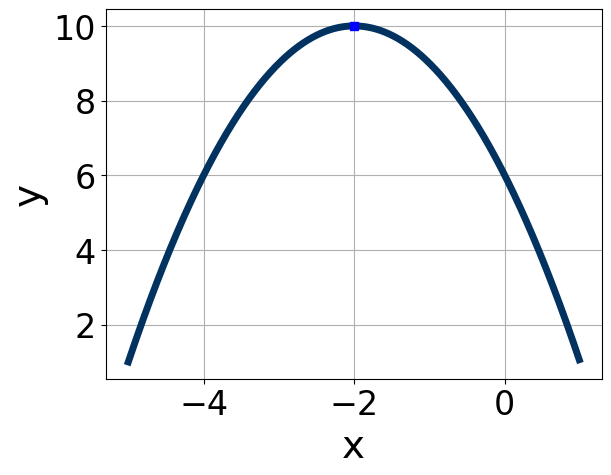
\includegraphics[width=0.5\textwidth]{../Figures/quadraticGraphToEquationCopyA.png}
\end{center}
\begin{enumerate}[label=\Alph*.]
\item \( a \in [-1.3, -0.9], \hspace*{5mm} b \in [3, 9], \text{ and } \hspace*{5mm} c \in [-6, -4] \)
\item \( a \in [0.9, 1.6], \hspace*{5mm} b \in [3, 9], \text{ and } \hspace*{5mm} c \in [0, 3] \)
\item \( a \in [-1.3, -0.9], \hspace*{5mm} b \in [-6, -3], \text{ and } \hspace*{5mm} c \in [-6, -4] \)
\item \( a \in [0.9, 1.6], \hspace*{5mm} b \in [-6, -3], \text{ and } \hspace*{5mm} c \in [5, 9] \)
\item \( a \in [0.9, 1.6], \hspace*{5mm} b \in [-6, -3], \text{ and } \hspace*{5mm} c \in [0, 3] \)

\end{enumerate} }
\litem{
Factor the quadratic below. Then, choose the intervals that contain the constants in the form $(ax+b)(cx+d); b \leq d.$\[ 24x^{2} -38 x + 15 \]\begin{enumerate}[label=\Alph*.]
\item \( a \in [17.94, 18.79], \hspace*{5mm} b \in [-7, 2], \hspace*{5mm} c \in [-0.3, 2.2], \text{ and } \hspace*{5mm} d \in [-5, -1] \)
\item \( a \in [4.74, 7.72], \hspace*{5mm} b \in [-7, 2], \hspace*{5mm} c \in [1.4, 4.8], \text{ and } \hspace*{5mm} d \in [-5, -1] \)
\item \( a \in [1.79, 4.46], \hspace*{5mm} b \in [-7, 2], \hspace*{5mm} c \in [4.9, 8.9], \text{ and } \hspace*{5mm} d \in [-5, -1] \)
\item \( a \in [0.82, 1.2], \hspace*{5mm} b \in [-27, -17], \hspace*{5mm} c \in [-0.3, 2.2], \text{ and } \hspace*{5mm} d \in [-19, -14] \)
\item \( \text{None of the above.} \)

\end{enumerate} }
\litem{
Solve the quadratic equation below. Then, choose the intervals that the solutions $x_1$ and $x_2$ belong to, with $x_1 \leq x_2$.\[ 25x^{2} -15 x -54 = 0 \]\begin{enumerate}[label=\Alph*.]
\item \( x_1 \in [-1.45, -0.63] \text{ and } x_2 \in [1.68, 1.81] \)
\item \( x_1 \in [-6.62, -5.24] \text{ and } x_2 \in [0.33, 0.42] \)
\item \( x_1 \in [-4.68, -3.42] \text{ and } x_2 \in [0.6, 0.86] \)
\item \( x_1 \in [-31.56, -29.49] \text{ and } x_2 \in [44.72, 45.21] \)
\item \( x_1 \in [-0.67, 0.57] \text{ and } x_2 \in [3.28, 3.94] \)

\end{enumerate} }
\litem{
Graph the equation below.\[ f(x) = -(x-1)^2 + 15 \]\begin{enumerate}[label=\Alph*.]
\begin{multicols}{2}\item 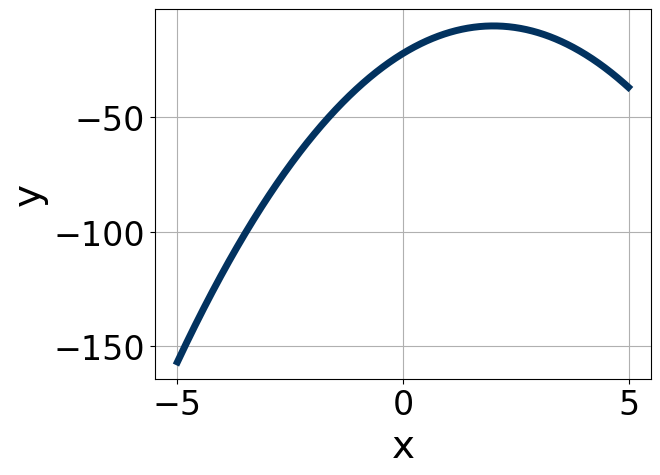
\includegraphics[width = 0.3\textwidth]{../Figures/quadraticEquationToGraphCopyAA.png}\item 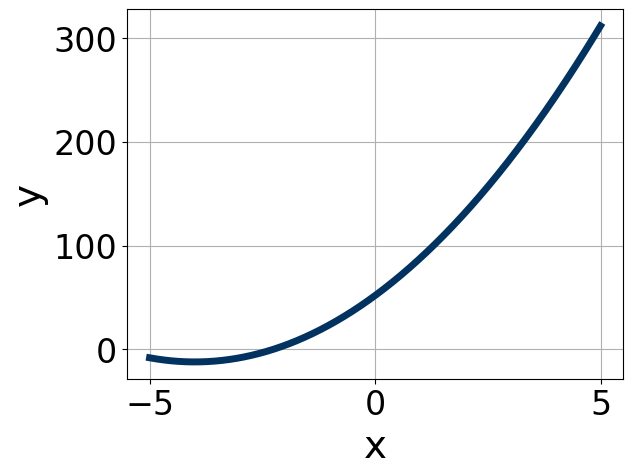
\includegraphics[width = 0.3\textwidth]{../Figures/quadraticEquationToGraphCopyBA.png}\item 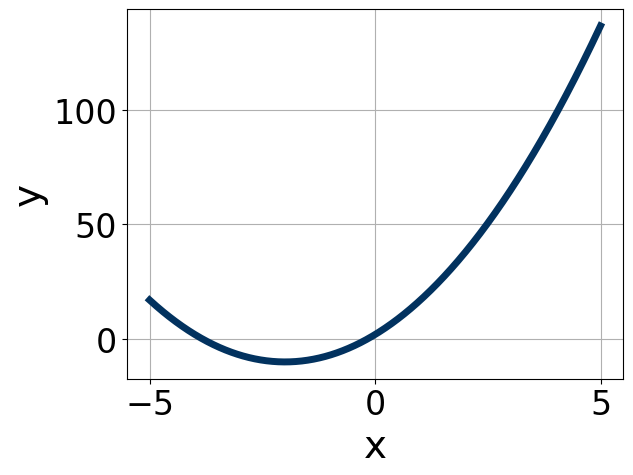
\includegraphics[width = 0.3\textwidth]{../Figures/quadraticEquationToGraphCopyCA.png}\item 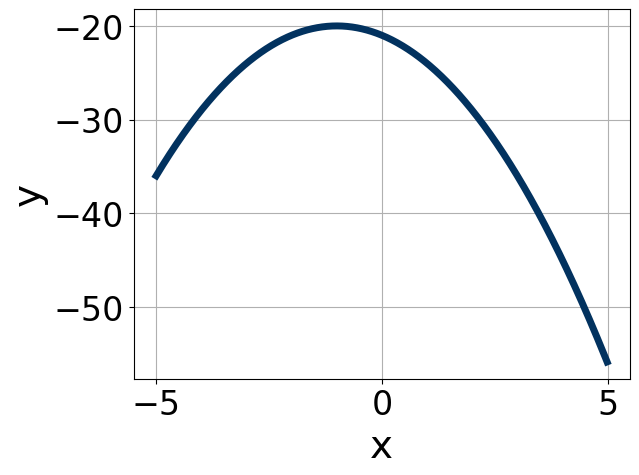
\includegraphics[width = 0.3\textwidth]{../Figures/quadraticEquationToGraphCopyDA.png}\end{multicols}\item None of the above.
\end{enumerate} }
\litem{
Graph the equation below.\[ f(x) = -(x-4)^2 + 16 \]\begin{enumerate}[label=\Alph*.]
\begin{multicols}{2}\item 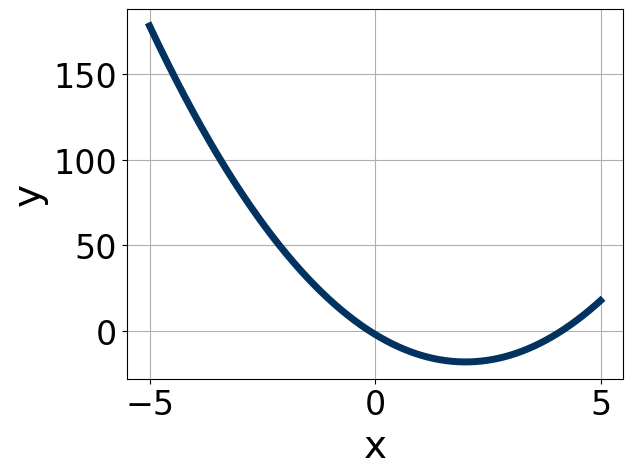
\includegraphics[width = 0.3\textwidth]{../Figures/quadraticEquationToGraphAA.png}\item 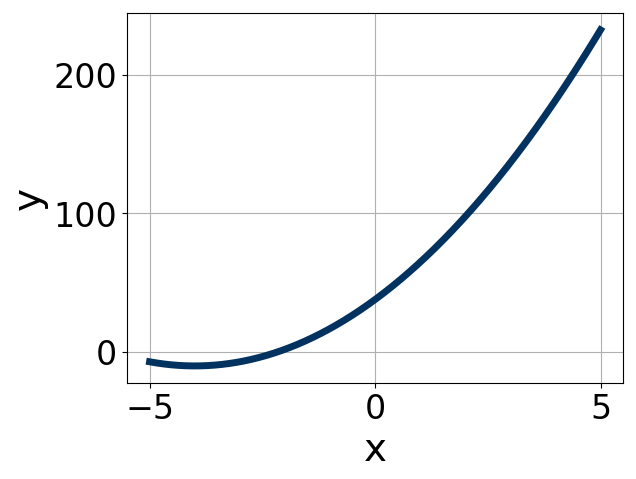
\includegraphics[width = 0.3\textwidth]{../Figures/quadraticEquationToGraphBA.png}\item 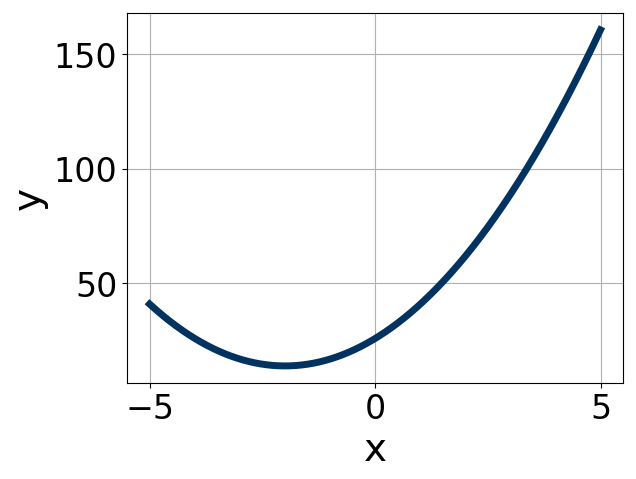
\includegraphics[width = 0.3\textwidth]{../Figures/quadraticEquationToGraphCA.png}\item 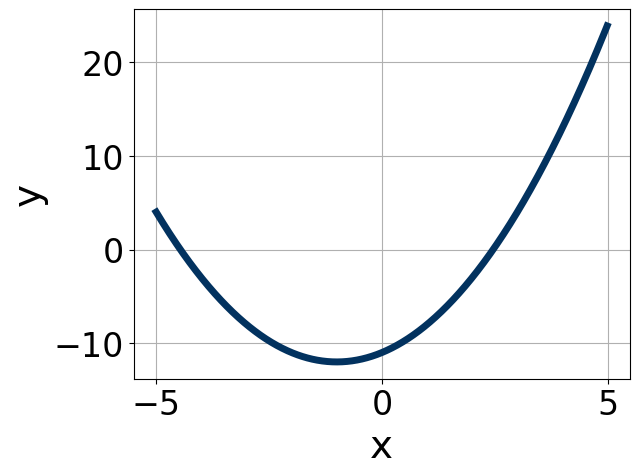
\includegraphics[width = 0.3\textwidth]{../Figures/quadraticEquationToGraphDA.png}\end{multicols}\item None of the above.
\end{enumerate} }
\litem{
Write the equation of the graph presented below in the form $f(x)=ax^2+bx+c$, assuming  $a=1$ or $a=-1$. Then, choose the intervals that $a, b,$ and $c$ belong to.
\begin{center}
    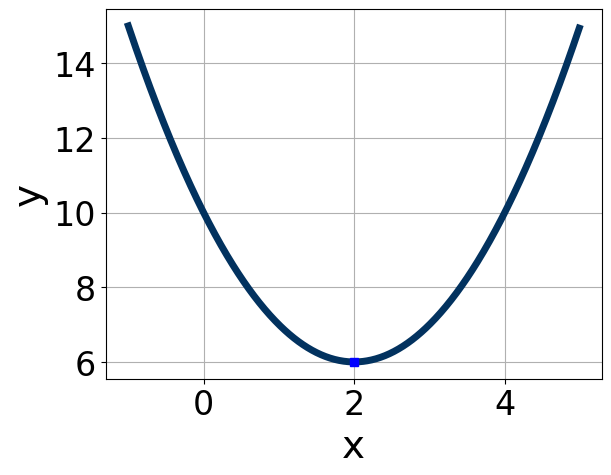
\includegraphics[width=0.5\textwidth]{../Figures/quadraticGraphToEquationA.png}
\end{center}
\begin{enumerate}[label=\Alph*.]
\item \( a \in [0.5, 2], \hspace*{5mm} b \in [-12, -5], \text{ and } \hspace*{5mm} c \in [23, 25] \)
\item \( a \in [0.5, 2], \hspace*{5mm} b \in [6, 11], \text{ and } \hspace*{5mm} c \in [23, 25] \)
\item \( a \in [-2.1, -0.7], \hspace*{5mm} b \in [-12, -5], \text{ and } \hspace*{5mm} c \in [-9, -7] \)
\item \( a \in [-2.1, -0.7], \hspace*{5mm} b \in [6, 11], \text{ and } \hspace*{5mm} c \in [-25, -22] \)
\item \( a \in [-2.1, -0.7], \hspace*{5mm} b \in [6, 11], \text{ and } \hspace*{5mm} c \in [-9, -7] \)

\end{enumerate} }
\litem{
Solve the quadratic equation below. Then, choose the intervals that the solutions $x_1$ and $x_2$ belong to, with $x_1 \leq x_2$.\[ 25x^{2} +50 x + 24 = 0 \]\begin{enumerate}[label=\Alph*.]
\item \( x_1 \in [-30.1, -29.93] \text{ and } x_2 \in [-20.14, -19.97] \)
\item \( x_1 \in [-6.07, -5.69] \text{ and } x_2 \in [-0.17, -0.13] \)
\item \( x_1 \in [-3.9, -3.37] \text{ and } x_2 \in [-0.36, -0.2] \)
\item \( x_1 \in [-1.77, -1.5] \text{ and } x_2 \in [-0.76, -0.52] \)
\item \( x_1 \in [-1.3, -1.1] \text{ and } x_2 \in [-1.07, -0.64] \)

\end{enumerate} }
\litem{
Factor the quadratic below. Then, choose the intervals that contain the constants in the form $(ax+b)(cx+d); b \leq d.$\[ 24x^{2} -2 x -15 \]\begin{enumerate}[label=\Alph*.]
\item \( a \in [12.7, 18.5], \hspace*{5mm} b \in [-8, -3], \hspace*{5mm} c \in [-1.8, 1.3], \text{ and } \hspace*{5mm} d \in [-1, 8] \)
\item \( a \in [3.3, 8], \hspace*{5mm} b \in [-8, -3], \hspace*{5mm} c \in [2, 4.4], \text{ and } \hspace*{5mm} d \in [-1, 8] \)
\item \( a \in [-2.3, 1.5], \hspace*{5mm} b \in [-20, -13], \hspace*{5mm} c \in [-1.8, 1.3], \text{ and } \hspace*{5mm} d \in [16, 21] \)
\item \( a \in [1.4, 5.6], \hspace*{5mm} b \in [-8, -3], \hspace*{5mm} c \in [6, 10.3], \text{ and } \hspace*{5mm} d \in [-1, 8] \)
\item \( \text{None of the above.} \)

\end{enumerate} }
\litem{
Solve the quadratic equation below. Then, choose the intervals that the solutions belong to, with $x_1 \leq x_2$ (if they exist).\[ -10x^{2} +13 x + 7 = 0 \]\begin{enumerate}[label=\Alph*.]
\item \( x_1 \in [-0.41, 0.59] \text{ and } x_2 \in [1.62, 1.72] \)
\item \( x_1 \in [-22.54, -18.54] \text{ and } x_2 \in [21.66, 22.01] \)
\item \( x_1 \in [-3.71, -0.71] \text{ and } x_2 \in [-0.19, 0.66] \)
\item \( x_1 \in [-19.09, -15.09] \text{ and } x_2 \in [3.63, 4.5] \)
\item \( \text{There are no Real solutions.} \)

\end{enumerate} }
\litem{
Solve the quadratic equation below. Then, choose the intervals that the solutions belong to, with $x_1 \leq x_2$ (if they exist).\[ 13x^{2} +13 x -2 = 0 \]\begin{enumerate}[label=\Alph*.]
\item \( x_1 \in [-19.9, -16.8] \text{ and } x_2 \in [15.32, 16.76] \)
\item \( x_1 \in [-16.2, -13.6] \text{ and } x_2 \in [1.45, 2.59] \)
\item \( x_1 \in [-1.8, -1] \text{ and } x_2 \in [-0.53, 0.25] \)
\item \( x_1 \in [-0.9, 2.9] \text{ and } x_2 \in [0.54, 1.56] \)
\item \( \text{There are no Real solutions.} \)

\end{enumerate} }
\end{enumerate}

\end{document}